\section{Synthetic Data Generation Pipelines}

\begin{frame}{}
    \LARGE Alignment and Post-Training: \textbf{Synthetic Data Pipelines}

    \vspace{1em}
    \normalsize If the model writes its own training data, what keeps the data good?
\end{frame}

\begin{frame}{Every Pipeline Is the Same Loop}
    \centering
    \begin{adjustbox}{max width=\linewidth}\begin{tikzpicture}[font=\small,
        st/.style={draw, rounded corners=2pt, minimum width=1.9cm, minimum height=0.95cm, align=center, fill=KAUSTcyan!15},
        arr/.style={-{Stealth}, thick}]
        \node[st, fill=gray!12] (s) at (0,0) {Seed\\{\scriptsize tasks, web text}};
        \node[st] (d) at (2.5,0) {Diversify\\{\scriptsize personas, styles}};
        \node[st] (g) at (5.0,0) {Generate\\{\scriptsize teacher or self}};
        \node[st, fill=darkorange!20] (v) at (7.5,0) {Verify\\{\scriptsize run, judge}};
        \node[st, fill=darkorange!20] (c) at (10.0,0) {Clean\\{\scriptsize dedup, decontam.}};
        \node[st, fill=gray!12] (m) at (12.5,0) {Mix\\{\scriptsize with real data}};
        \draw[arr] (s) -- (d);
        \draw[arr] (d) -- (g);
        \draw[arr] (g) -- (v);
        \draw[arr] (v) -- (c);
        \draw[arr] (c) -- (m);
        \draw[arr, KAUSTblue, dashed] (c.south) -- ++(0,-0.3) -| (s.south);
        \node[font=\scriptsize, KAUSTblue] at (5.0,-1.15) {survivors return to the seed pool};
    \end{tikzpicture}\end{adjustbox}
    \vspace{0.3em}
    \begin{itemize}\itemsep0.45em
        \item \textbf{Why it took over.} Nemotron-4 340B: more than 98\% of alignment data is synthetic, with about 20K human-annotated samples. Phi-4: 40\% of \emph{pre-training} tokens are synthetic.
        \item \textbf{What varies between pipelines} is where the effort goes. Early work spent it on \emph{generate}. Current work spends it on \emph{diversify} and \emph{verify}.
        \item We follow the loop from left to right, then ask what happens when it runs for many generations.
    \end{itemize}
    \src{NVIDIA, ``Nemotron-4 340B Technical Report,'' \href{https://arxiv.org/abs/2406.11704}{arXiv:2406.11704}. Microsoft, ``Phi-4 Technical Report,'' \href{https://arxiv.org/abs/2412.08905}{arXiv:2412.08905}, Table 5. Loop after Liu et al., ``Best Practices and Lessons Learned on Synthetic Data,'' \href{https://arxiv.org/abs/2404.07503}{arXiv:2404.07503}.}
\end{frame}

\begin{frame}{The Lineage, 2022 to 2023}
    \begin{center}
    \small
    \begin{adjustbox}{max width=\linewidth}\begin{tabular}{l>{\raggedright\arraybackslash}p{5.6cm}>{\raggedright\arraybackslash}p{5.0cm}}
        \toprule
        \textbf{Pipeline} & \textbf{New idea} & \textbf{Scale and result} \\
        \midrule
        Self-Instruct & bootstrap from 175 seed tasks, filter near-duplicates by ROUGE-L & 52K instructions. SuperNI score of GPT-3 from 6.8 to 39.9 \\
        Alpaca & a simplified Self-Instruct loop with text-davinci-003 as teacher &52K demonstrations for under 500 dollars \\
        Evol-Instruct & rewrite each prompt to be deeper or broader & 52K to 250K in four rounds \\
        UltraFeedback & synthetic \emph{preferences}: GPT-4 rates 4 of 17 models per prompt & 64K prompts, over 1M feedback items \\
        \bottomrule
    \end{tabular}\end{adjustbox}
    \end{center}
    \begin{itemize}\itemsep0.4em
        \item A number worth remembering: only \alert{54\%} of Self-Instruct examples were fully valid. The model improved by 33 points anyway.
        \item \textbf{Instruction tuning tolerates noise.} Pre-training data does not: it needs high-quality synthetic text.
    \end{itemize}
    \src{Wang et al., ``Self-Instruct,'' ACL 2023, \href{https://arxiv.org/abs/2212.10560}{arXiv:2212.10560}. Taori et al., ``Alpaca'' (Stanford CRFM, 2023). Xu et al., ``WizardLM,'' \href{https://arxiv.org/abs/2304.12244}{arXiv:2304.12244}. Cui et al., \href{https://arxiv.org/abs/2310.01377}{arXiv:2310.01377}. Yan, ``How to Generate and Use Synthetic Data for Finetuning'' (2024).}
\end{frame}

\begin{frame}{Diversity for Almost Nothing: Magpie and Persona Hub}
    \centering
    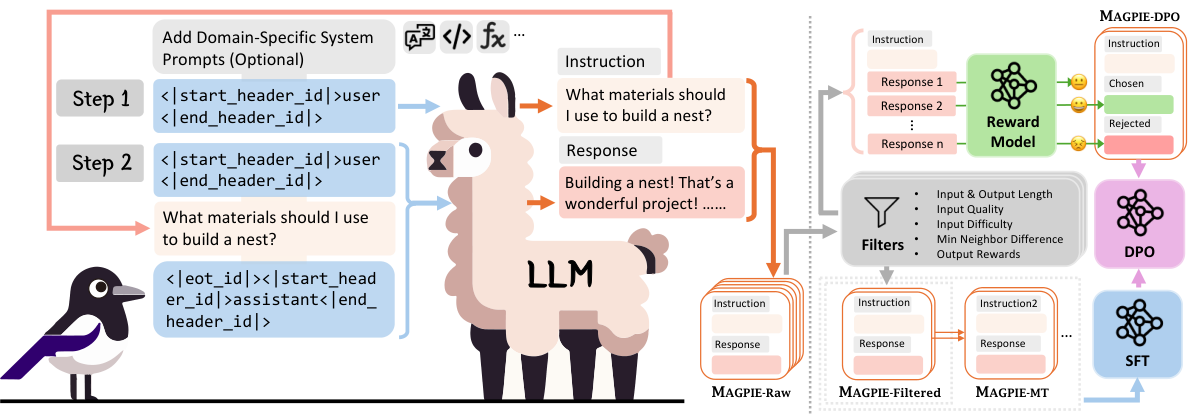
\includegraphics[width=0.74\linewidth,height=0.38\textheight,keepaspectratio]{images/alignment-post-training/magpie_fig1_pipeline.png}
    \begin{itemize}\itemsep0.3em
        \item \textbf{Magpie.} Give an aligned model only the \emph{pre-query template}, the tokens that open a user turn. It writes a user query by itself. No seeds, no prompt engineering.
        \item 3M instructions in 206 GPU-hours. SFT on a filtered 300K subset beats the official Llama-3-8B-Instruct on AlpacaEval 2, but is weaker on maths.
        \item \textbf{Persona Hub.} One billion personas, built by asking ``who is likely to read, write, like or dislike this text?''. T\"ulu 3 builds its skill data from 250K of them.
    \end{itemize}
    \src{Xu et al., ``Magpie,'' ICLR 2025, \href{https://arxiv.org/abs/2406.08464}{arXiv:2406.08464}, Figure 1 and Table 1. Ge et al., ``Scaling Synthetic Data Creation with 1,000,000,000 Personas,'' \href{https://arxiv.org/abs/2406.20094}{arXiv:2406.20094}. T\"ulu 3, \href{https://arxiv.org/abs/2411.15124}{arXiv:2411.15124}.}
\end{frame}

\begin{frame}{Frontier Recipes: Verify What the Model Wrote Itself}
    \begin{columns}[T,onlytextwidth]
        \column{0.55\textwidth}
        \begin{itemize}\itemsep0.45em
            \item \textbf{Nemotron-4: a flywheel.} Each aligned model becomes the next generator. Intermediate checkpoints surpassed their teachers.
            \item \textbf{Llama 3: execution feedback.} About 1M code examples pass static analysis and generated unit tests. Training the 405B model on its own generations \alert{without} this check did not help.
            \item \textbf{Phi-4: synthetic pre-training.} More epochs over synthetic data beat adding fresh web tokens (right). But models trained on synthetic data \emph{alone} hallucinated more.
        \end{itemize}
        \column{0.43\textwidth}
        \centering
        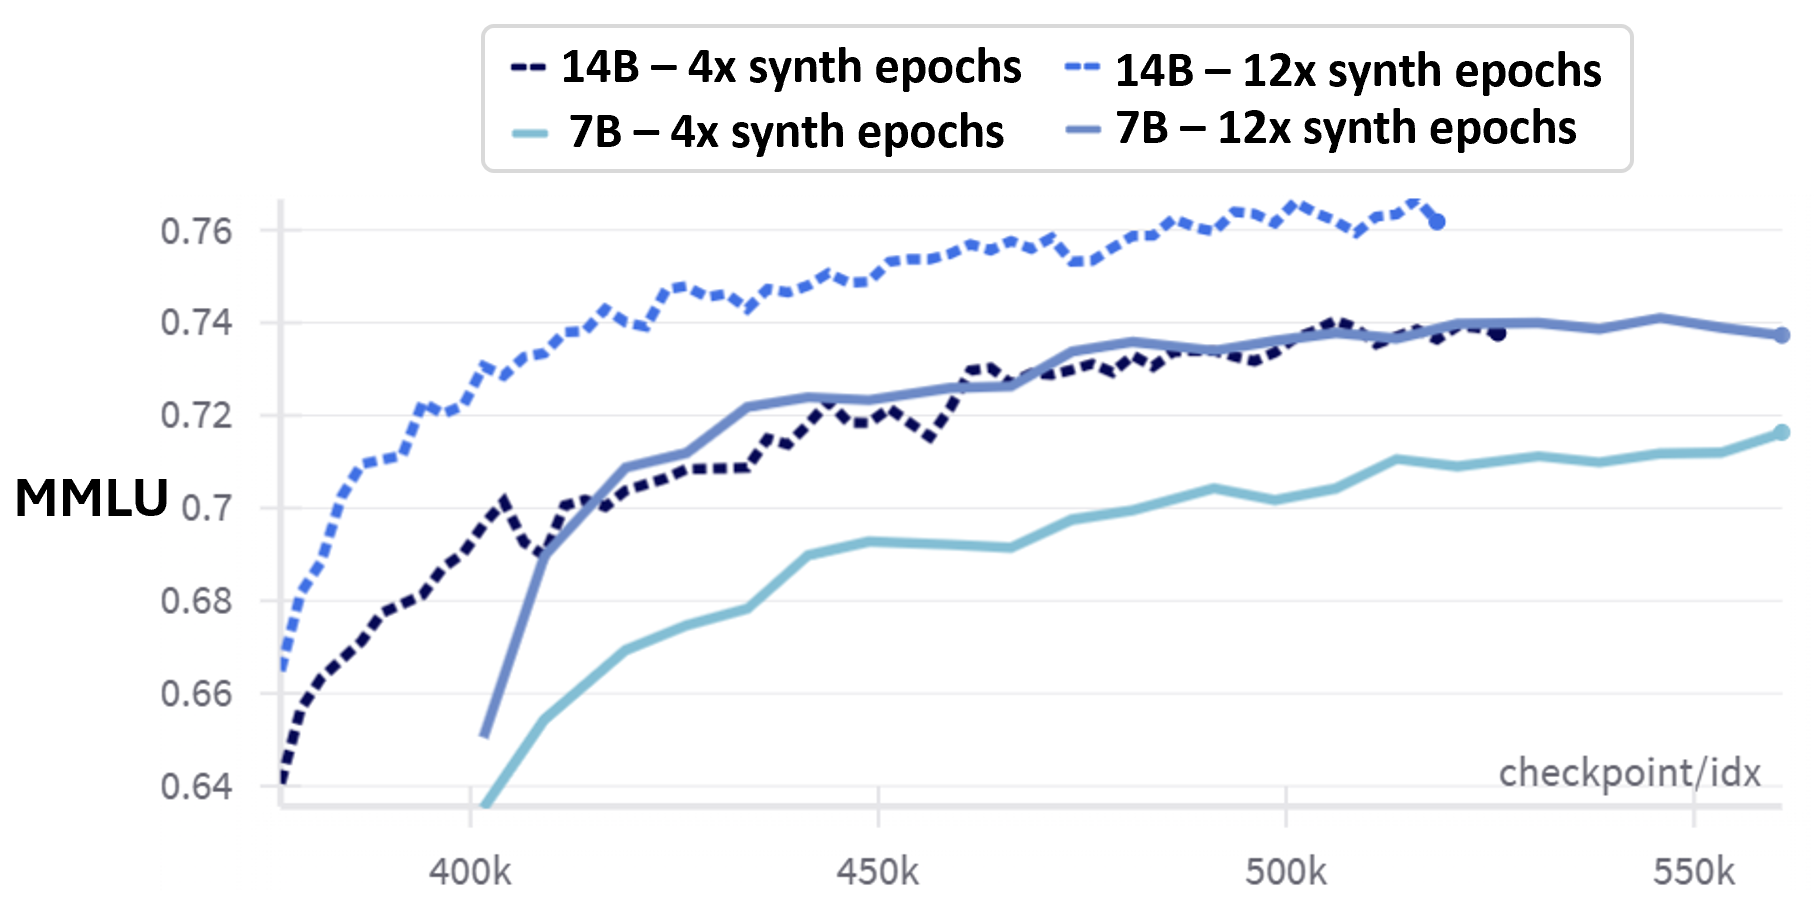
\includegraphics[width=\linewidth,height=0.5\textheight,keepaspectratio]{images/alignment-post-training/phi4_fig2_synth_epochs.png}
    \end{columns}
    \vspace{0.2em}
    \src{NVIDIA, \href{https://arxiv.org/abs/2406.11704}{arXiv:2406.11704}. Meta, ``The Llama 3 Herd of Models,'' \href{https://arxiv.org/abs/2407.21783}{arXiv:2407.21783}, Sec. 4.2 to 4.3. Microsoft, ``Phi-4 Technical Report,'' \href{https://arxiv.org/abs/2412.08905}{arXiv:2412.08905}, Figure 2.}
\end{frame}

\begin{frame}{Reasoning Traces: Less Is More, or More Is More?}
    \begin{center}
    \small
    \begin{adjustbox}{max width=\linewidth}\begin{tabular}{l>{\raggedright\arraybackslash}p{2.3cm}>{\raggedright\arraybackslash}p{5.6cm}>{\raggedright\arraybackslash}p{3.3cm}}
        \toprule
        \textbf{Dataset} & \textbf{Size} & \textbf{Selection rule} & \textbf{Result} \\
        \midrule
        s1K & 1,000 of 59K & keep what both a 7B and a 32B model fail, then spread over 50 domains & AIME24 50.0 (32B student) \\
        LIMO & 800 of 2,125 & keep problems a strong model solves in only 1 to 3 of 32 attempts & AIME24 63.3 (32B student) \\
        OpenThoughts3 & 1.2M & LLM difficulty labels, 16 answers per question & AIME25 53 (7B student) \\
        \bottomrule
    \end{tabular}\end{adjustbox}
    \end{center}
    \begin{itemize}\itemsep0.4em
        \item \textbf{Two regimes.} A few hundred traces suffice when the base model already has the knowledge. A small student needs a million. \textbf{Both rely on difficulty filtering.}
        \item \textbf{Two surprises.} A weaker model (QwQ-32B) was the better teacher. And no answer-filtering strategy beat keeping every answer of a strong teacher.
    \end{itemize}
    \src{Muennighoff et al., ``s1: Simple test-time scaling,'' \href{https://arxiv.org/abs/2501.19393}{arXiv:2501.19393}. Ye et al., ``LIMO: Less is More for Reasoning,'' \href{https://arxiv.org/abs/2502.03387}{arXiv:2502.03387}. Guha, Marten et al., ``OpenThoughts: Data Recipes for Reasoning Models,'' \href{https://arxiv.org/abs/2506.04178}{arXiv:2506.04178}.}
\end{frame}

\begin{frame}{The Quality-Control Ladder}
    \begin{center}
    \small
    \begin{adjustbox}{max width=\linewidth}\begin{tabular}{l>{\raggedright\arraybackslash}p{4.3cm}>{\raggedright\arraybackslash}p{6.6cm}}
        \toprule
        \textbf{Rung} & \textbf{Signal} & \textbf{Used by} \\
        \midrule
        \rowcolor{KAUSTcyan!12} 1. Verifier & execution, unit tests, constraint checkers & Llama 3 code data, Phi-4, T\"ulu 3 verifiable rewards \\
        2. Reward model & learned score & Llama 3 top quartile, Nemotron-4 reward-model-as-judge \\
        3. LLM judge & rubric, rated jointly & UltraFeedback, Magpie quality and difficulty tags \\
        4. Heuristics & overlap, length, keywords & Self-Instruct (ROUGE-L below 0.7), MinHash at 0.9 \\
        \bottomrule
    \end{tabular}\end{adjustbox}
    \end{center}
    \begin{itemize}\itemsep0.4em
        \item \textbf{Climb as high as the task allows.} Verifiers first, heuristics last.
        \item \textbf{Do not trust a single judge.} In Llama 3 the reward model and the LLM judge often disagreed. Taking the union of their picks gave the best recall.
    \end{itemize}
    \src{Sources as on the previous slides. Liu et al., \href{https://arxiv.org/abs/2404.07503}{arXiv:2404.07503}. Chen et al., ``On the Diversity of Synthetic Data and its Impact on Training LLMs,'' \href{https://arxiv.org/abs/2410.15226}{arXiv:2410.15226}. Ordering of the rungs is a synthesis.}
\end{frame}

\begin{frame}{Model Collapse, Stated Carefully}
    \begin{columns}[T,onlytextwidth]
        \column{0.55\textwidth}
        \begin{itemize}\itemsep0.25em
            \item \textbf{The \emph{Nature} result.} Train each generation only on the previous one's output. First the tails vanish, then the variance.
            \item Keeping \textbf{10\% original data} leaves only minor degradation.
            \item \textbf{Replace or accumulate?} For linear regression, test error after $n$ generations is
        \end{itemize}
        {\footnotesize\[
            E_{\text{replace}}=\frac{\sigma^2 d}{T-d-1}\,n,
            \qquad
            E_{\text{accum}}=\frac{\sigma^2 d}{T-d-1}\sum_{i=1}^{n}\frac{1}{i^2}
        \]}
        \begin{itemize}\itemsep0.4em
            \item The sum is bounded by $\pi^2/6$. Error explodes only if old data is thrown away.
        \end{itemize}
        \column{0.43\textwidth}
        \centering
        \begin{adjustbox}{max width=\linewidth}\begin{tikzpicture}
            \begin{axis}[width=6.4cm, height=4.8cm, xmin=1, xmax=10, ymin=0, ymax=10,
                xlabel={\scriptsize generation $n$}, ylabel={\scriptsize scaled test error},
                tick label style={font=\scriptsize}, axis lines=left,
                legend style={font=\scriptsize, draw=none, at={(0.03,0.97)}, anchor=north west}]
                \addplot[KAred, thick, mark=*, mark size=1.2pt] coordinates {(1,1) (2,2) (3,3) (4,4) (5,5) (6,6) (7,7) (8,8) (9,9) (10,10)};
                \addplot[KAUSTblue, thick, mark=square*, mark size=1.2pt] coordinates {(1,1) (2,1.25) (3,1.361) (4,1.424) (5,1.464) (6,1.491) (7,1.512) (8,1.527) (9,1.540) (10,1.550)};
                \legend{replace, accumulate}
            \end{axis}
        \end{tikzpicture}\end{adjustbox}
    \end{columns}
    \vspace{0.2em}
    \takeaway{Collapse comes from \textbf{replacing} real data, not from synthetic data as such.}
    \src{Shumailov et al., ``AI models collapse when trained on recursively generated data,'' \emph{Nature} 631 (2024). Gerstgrasser et al., ``Is Model Collapse Inevitable?'' \href{https://arxiv.org/abs/2404.01413}{arXiv:2404.01413}, Eqs. 3 to 4 (curves plotted from these).}
\end{frame}

\begin{frame}{The Live Risk Is Diversity, Not Collapse}
    \begin{center}
    \small
    \begin{adjustbox}{max width=\linewidth}\begin{tabular}{>{\raggedright\arraybackslash}p{3.4cm}>{\raggedright\arraybackslash}p{10.0cm}}
        \toprule
        \textbf{Study} & \textbf{Finding} \\
        \midrule
        Taori and Hashimoto (2022) & A dataset is 70\% female, the model predicts 90\%, and after 16 rounds of self-labelling 97\%. Beam search amplifies far more than sampling \\
        Guo et al. (2024) & Syntactic diversity halves over six recursive rounds. A quality filter that drops the worst 20\% \alert{made it worse} \\
        Kova\v{c} et al. (2025) & Dose-response: almost no shift at 1/16 synthetic, a plateau from 1/2 upward \\
        Karouzos et al. (2026) & In the Olmo 3 lineages, reasoning SFT loses 62\% of semantic diversity. The RL-Zero lineage keeps at least 71\% \\
        \bottomrule
    \end{tabular}\end{adjustbox}
    \end{center}
    \begin{itemize}\itemsep0.4em
        \item \textbf{Amplification follows from calibration.} A generator that \emph{samples} stays bounded. One that takes the argmax, or is distilled narrowly, compresses the distribution.
        \item \textbf{Mitigations, in order:} sample instead of searching, cap the synthetic share, rebalance with stratified or counterfactual data. Do not rely on quality filters.
    \end{itemize}
    \src{Taori, Hashimoto, ``Data Feedback Loops,'' \href{https://arxiv.org/abs/2209.03942}{arXiv:2209.03942}. Guo et al., \href{https://arxiv.org/abs/2311.09807}{arXiv:2311.09807}. Kova\v{c} et al., ``Recursive Training Loops in LLMs,'' \href{https://arxiv.org/abs/2504.03814}{arXiv:2504.03814}. Karouzos, Tan, Aletras, \href{https://arxiv.org/abs/2604.16027}{arXiv:2604.16027}.}
\end{frame}

\begin{frame}{May You Distil That Model? Terms in 2026}
    \begin{center}
    \small
    \begin{adjustbox}{max width=\linewidth}\begin{tabular}{l>{\raggedright\arraybackslash}p{10.2cm}}
        \toprule
        \textbf{Teacher} & \textbf{What the terms say about training on outputs} \\
        \midrule
        OpenAI API & using output ``to develop models that compete with OpenAI'' is prohibited \\
        Anthropic API & no access ``to build a competing product or service, including to train competing AI models'' \\
        Llama 3.1 & allowed, but a model trained on its outputs must carry a name starting with ``Llama'' \\
        \rowcolor{KAUSTcyan!12} Nemotron-4 & licence explicitly permits synthetic data generation \\
        \bottomrule
    \end{tabular}\end{adjustbox}
    \end{center}
    \begin{itemize}\itemsep0.4em
        \item The Gemini API terms have the same clause. \textbf{Enforcement is real:} in February 2026 Anthropic reported over 16 million exchanges across about 24,000 fraudulent accounts used for distillation, and named three labs.
        \item The binding constraint on distilling a closed model is \textbf{contract and enforcement}, not copyright. Permissive open-weight teachers are the clean route.
    \end{itemize}
    \src{OpenAI Terms of Use (Jan 2026, read through a proxy reader: confirm the wording before quoting). Anthropic Commercial Terms (Jun 2025). Llama 3.1 Community License. Anthropic, ``Detecting and preventing distillation attacks'' (Feb 2026).}
\end{frame}

\begin{frame}{Synthetic Data: What to Remember}
    \begin{itemize}\itemsep0.6em
        \item One loop: seed, diversify, generate, verify, clean, mix. Effort has moved from generation to \textbf{diversity} and \textbf{verification}.
        \item Diversity is cheap now: template prompting and personas. Verification is not, and it matters most when a model learns from \textbf{its own} outputs.
        \item Model collapse needs replacement. What actually erodes is \textbf{diversity}, and quality filters make that worse.
        \item 2026 direction: the line between pre-training and post-training data is blurring. One fully synthetic corpus, grown from 58,698 Wikipedia articles, trains a model in a single stage with 10 to 140 times fewer tokens.
    \end{itemize}
    \vspace{0.3em}
    \takeaway{\textbf{Next.} Synthetic data still starts from real text. How is the real corpus chosen, when the raw pool is hundreds of trillions of tokens?}
    \src{Langlais et al., ``It's All Training: A Fully Synthetic Single-Stage Recipe for LLMs,'' \href{https://arxiv.org/abs/2609.37891}{arXiv:2609.37891} (abstract).}
\end{frame}
